% Class Notes Template
\documentclass[12pt]{article}
\usepackage[margin=1in]{geometry} 
\usepackage[utf8]{inputenc}

% Packages
\usepackage[french, english]{babel}
\usepackage{amsmath, amsthm, amssymb ,amsfonts, graphics, tikz, float, enumerate}
\usepackage{listings}
\usepackage{color} %red, green, blue, yellow, cyan, magenta, black, white
\definecolor{mygreen}{RGB}{28,172,0} % color values Red, Green, Blue
\definecolor{mylilas}{RGB}{170,55,241}

\lstset{language=Matlab,%
	%basicstyle=\color{red},
	breaklines=true,%
	morekeywords={matlab2tikz},
	keywordstyle=\color{blue},%
	morekeywords=[2]{1}, keywordstyle=[2]{\color{black}},
	identifierstyle=\color{black},%
	stringstyle=\color{mylilas},
	commentstyle=\color{mygreen},%
	showstringspaces=false,%without this there will be a symbol in the places where there is a space
	numbers=left,%
	numberstyle={\tiny \color{black}},% size of the numbers
	numbersep=9pt, % this defines how far the numbers are from the text
	emph=[1]{for,end,break},emphstyle=[1]\color{blue}, %some words to emphasise
	%emph=[2]{word1,word2}, emphstyle=[2]{style},    
}

% Title
\title{ECON 6130 - Problem Set \# 2}
\date{\today}
\author{Julien Manuel Neves}

% Use these for theorems, lemmas, proofs, etc.
\theoremstyle{definition}
\newtheorem{example}{Example}[section]
\newtheorem{theorem}{Theorem}
\newtheorem{lemma}[theorem]{Lemma}
\newtheorem{proposition}[theorem]{Proposition}
\newtheorem{claim}[theorem]{Claim}
\newtheorem{axiom}[theorem]{Axiom}
\newtheorem{corollary}[theorem]{Corollary}
\newtheorem{remark}[theorem]{Remark}
\newtheorem{definition}[theorem]{Definition}

% Usefuls Macros
\newcommand\N{\mathbb{N}}
\newcommand\E{\mathbb{E}}
\newcommand\R{\mathbb{R}}
\newcommand\F{\mathcal{F}}
\newcommand\Z{\mathbb{Z}}
\newcommand\st{\text{ such that }}
\newcommand\seq[1]{\{ #1 \}}
\newcommand{\inv}{^{-1}}


\newcommand{\norm}[1]{\|#1 \|}
\newcommand{\inp}[2]{\langle #1, #2 \rangle}

\newcommand{\pa}[1]{\left(#1\right)}
\newcommand{\bra}[1]{\left[#1\right]}
\newcommand{\cbra}[1]{\left\{#1\right\}}

\newcommand{\pfrac}[2]{\pa{\frac{#1}{#2}}}
\newcommand{\bfrac}[2]{\bra{\frac{#1}{#2}}}

\newcommand{\mat}[1]{\begin{matrix}#1\end{matrix}}
\newcommand{\pmat}[1]{\pa{\mat{#1}}}
\newcommand{\bmat}[1]{\bra{\mat{#1}}}


\begin{document}

\maketitle

\section*{Part (a)}

Note that the equations for the New Keynesian business cycle can be listed as follows
\begin{align*}
\pi_t-\beta \E_t(\pi_{t+1}) -\kappa \tilde{y}_t	& = 0\\
 \tilde{y}_t - \E_t( \tilde{y}_{t+1}) + \frac{1}{\sigma}[(i_t-\rho)- \E_t(\pi_{t+1})-(r_t^n-\rho)]	& = 0\\
(i_t-\rho) -\phi_{\pi}\pi_t -\phi_y\tilde{y}_t - \phi_y\psi_{ya} a_t-v_t	& = 0\\
	(r_t^n-\rho) +\sigma(1-\rho_a)\psi_{ya}a_t -(1-\rho_z)z_t	& = 0\\
	v_t& = \rho_v v_{t-1} +\epsilon_t^v \\
	a_t& = \rho_a a_{t-1}+\epsilon_t^a \\
	z_t& = \rho_z z_{t-1}+\epsilon_t^z \\
	\tilde{y}_{t}& =\E_{t-1}(\tilde{y}_{t})+\eta_t^{\tilde{y}_t}\\
	\pi_{t}& = \E_{t-1}(\pi_{t})+ \eta_t^{\tilde{n}} 
\end{align*}
where $\eta_t$ are the forecast errors.

Thus, we define the following state space for our model
\[
S_t = [\tilde{y}_t,\pi_t,r_t^n-\rho,i_t-\rho,v_t,a_t,z_t,\E_t(\tilde{y}_{t+1}),\E_t(\pi_{t+1})]
\]

Note that the gensys.m code solves the following linear equation
\[
\Gamma_0 S_t = \Gamma_1 S_{t-1} + B +\Psi \epsilon_t + \Pi \eta_t
\]
where $E(\epsilon_t\epsilon_t')=I$.

Therefore, by rewriting the set of equations for the New Keynesian business cycle in matrix form, we get
\begin{align*}
\Gamma_0 &= \bmat{-\kappa & 1 & 0 &0 &0 &0 &0 &0 &-\beta\\
1& 0& -\frac{1}{\sigma}&  \frac{1}{\sigma} & 0 &0 &0 &-1& -\frac{1}{\sigma}\\
-\phi_y & -\phi_{\pi} & 0& 1& -1& -\phi_y\psi_{ya} &0& 0& 0\\
0 &0 &1 &0& 0& \sigma(1-\rho_a)\psi_{ya}& -(1-\rho_z) &0 &0\\
0 &0 &0 &0 &1 &0& 0& 0 &0\\
0 &0 &0 &0 &0 &1 &0 &0 &0\\
0 &0 &0 &0 &0 &0 &1 &0 &0\\
1 &0 &0 &0 &0 &0 &0 &0 &0\\
0 &1 &0 &0 &0 &0 &0 &0& 0}\\
\Gamma_1 &= \bmat{0 &0 &0& 0& 0& 0& 0& 0& 0\\
0 &0& 0& 0& 0& 0 &0& 0 &0\\
0 &0& 0& 0& 0 &0 &0 &0& 0\\
0 &0& 0& 0& 0 &0 &0 &0 &0\\
0 &0& 0& 0& \rho_v &0& 0& 0& 0\\
0 &0& 0& 0& 0 &\rho_a& 0& 0 &0\\
0 &0& 0& 0& 0& 0 &\rho_z& 0 &0\\
0 &0& 0& 0& 0& 0& 0 &1 &0\\
0 &0& 0& 0& 0 &0 &0& 0& 1}\\
\Psi    &= \bmat{0 &0& 0 &0 &\sigma_v &0& 0& 0& 0\\
0 &0& 0& 0& 0& \sigma_a &0& 0& 0\\
0 &0& 0& 0& 0& 0& \sigma_z& 0& 0}'\\
\Pi     &= \bmat{0& 0 &0 &0& 0& 0& 0& 1& 0\\
0& 0& 0& 0& 0& 0& 0& 0& 1}'\\
B   &= \bmat{0& 0& 0& 0& 0& 0& 0& 0& 0}'
\end{align*}

Then the gensys.m will ouput the coefficients of an $VAR(1)$ process of the following form
\[
S_t = A S_{t-1} + C \epsilon_t
\]
where $\epsilon_t\sim N(0,I)$.

Given the parameters of set in the problem set, we have
\begin{align*}
A &= \bmat{0  &  0        &0&   0&   -0.2684 &  -0.4039  &  0.1331 &   0 & 0\\
0   & 0       & 0 &  0 &  -0.0974 &  -0.3561  &  0.0795  & 0 &	0\\
0 &   0      &  0  & 0  & 0  & -0.2723   & 0.2100   & 0 &	0\\
0  &  0     &   0&   0 &  0.2196  & -0.3956   & 0.1858 &  0& 	0\\
0   & 0    &    0 &  0&    0.5000  & 0 &  0 &  0	&0\\
0 &   0   &     0  & 0 &  0  &  0.8000  &  0  & 0 &	0\\
0  &  0  &      0&   0  &  0  &  0 &   0.7000  &  0 	&0\\
0   & 0 &       0 &  0 &  -0.1342  & -0.3231  &  0.0932  &  0 &	0\\
0   & 0&        0  & 0  & -0.0487  & -0.2849 &   0.0556  & 0 &	0}\\
C & = \bmat{ -0.0054 &  -0.0040 &   0.0057\\
-0.0019  & -0.0036 &   0.0034\\
0  & -0.0027  &  0.0090\\
0.0044   &-0.0040 &   0.0080\\
0.0100   &0 &   0\\
0   & 0.0080   & 0\\
0   & 0 &   0.0300\\
-0.0027  & -0.0032  &  0.0040\\
-0.0010   &-0.0028 &   0.0024}
\end{align*}


\section*{Part (b)}

The impulse responses for inflation, output, output gap, interest rates and labor in responses to productivity, monetary policy and demand shocks are plotted in Fig.\ref{fig:impulse_monetary}, Fig.\ref{fig:impulse_prod} and Fig.\ref{fig:impulse_demand}.

Note that the impulses responses are consistent with the results shown in class.
\begin{figure}[H]
	\centering
	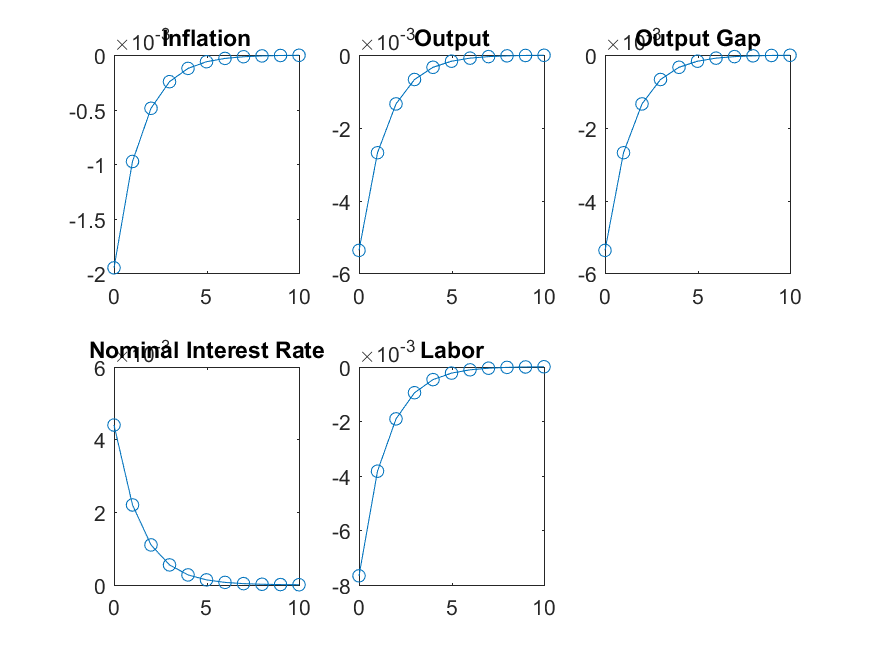
\includegraphics[width=\linewidth, height=0.4\textheight]{impulse_monetary}
	\caption{Impulse response to monetary shocks}
	\label{fig:impulse_monetary}
\end{figure}
\begin{figure}[H]
	\centering
	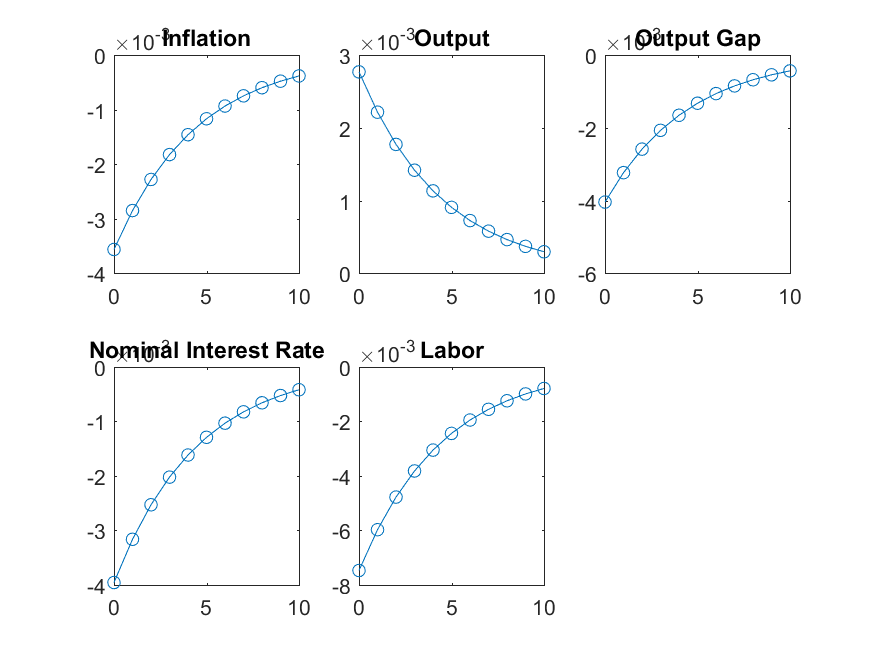
\includegraphics[width=\linewidth, height=0.4\textheight]{impulse_prod}
	\caption{Impulse response to productivity shocks}
	\label{fig:impulse_prod}
\end{figure}
\begin{figure}[H]
	\centering
	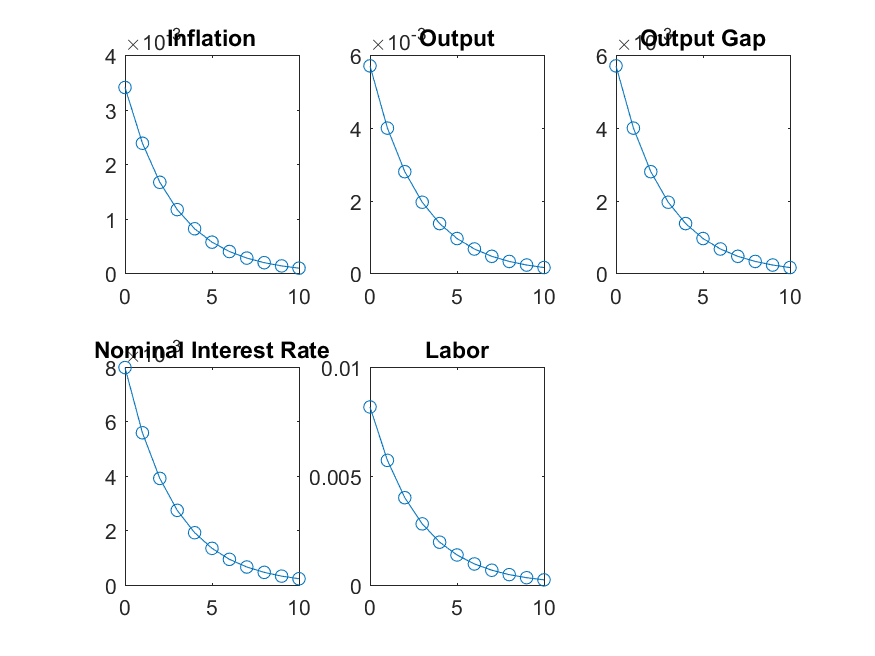
\includegraphics[width=\linewidth, height=0.4\textheight]{impulse_demand}
	\caption{Impulse response to demand shocks}
	\label{fig:impulse_demand}
\end{figure}

\section*{Part (c)}

Note that the nominal interest rates and inflation are included in our states $S_t$. As for output, we need to compute it using the following formula
\begin{align*}
\hat{y}_t &= y_t-y\\
&= (y_t-y_t^n)+(y_t^n-y)\\
&= \tilde{y}_t+\hat{y}^n_t\\
&= \tilde{y}_t+\psi_{ya}a_t
\end{align*}
where $y^n$, $y$, $\psi_{ya}$ and $a_t$ are defined as in Gali's book. 

Then, we can write inflation, output and nominal interest rates in the following matrix form
\[
Z(t) = DX(t)
\]
where 
\[
D = \bmat{0& 1& 0& 0& 0& 0& 0& 0& 0\\
	1& 0& 0& 0& 0& \psi_{ya}& 0& 0& 0\\
	0 &0& 0& 1& 0& 0& 0& 0& 0}
\]

The simulated inflation, output and nominal interest rates are plotted in Fig.\ref{fig:simulation}. The standard deviations are reported in part (d) and Tab.\ref{tab:sigma}.

\begin{figure}[H]
	\centering
	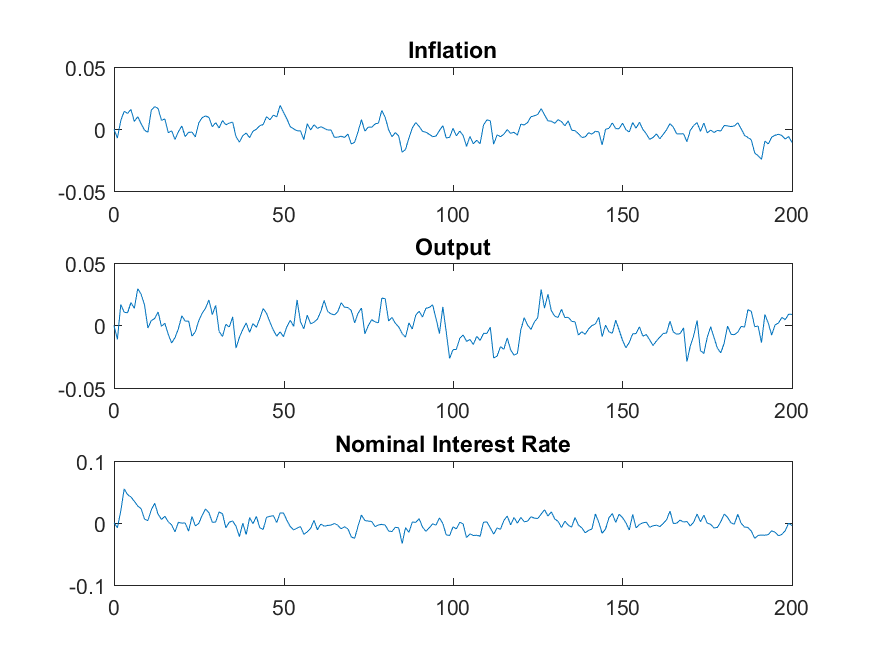
\includegraphics[width=\linewidth]{simulation}
	\caption{Simulation of New Keynesian business cycle model}
	\label{fig:simulation}
\end{figure}
\section*{Part (d)}

We use the following FRED series for our data:
\begin{enumerate}[(i)]
	\item Consumer Price Index of All Items in United States (USACPIALLQINMEI)
	\item Real Gross Domestic Product (GDPC1)
	\item Immediate Rates: Less than 24 Hours: Federal Funds Rate for the United States (IRSTFR01USQ156N)
\end{enumerate} 

Note that to compare the data to our model with need to log-linearized the series and detrend them using the Hodrick–Prescott filter. While the correspondence with the model states for GDP and the Federal Funds Rate is straightforward, it is important to note that the Consumer Price Index represents are price level. Therefore, after taking the log of the CPI, it is important to differentiate it before detrending it since
\[
\pi_t = \log(P_t)-\log(P_{t-1})
\]
where $P_t$ is the price level (CPI) at time $t$.


The sample inflation, output and nominal interest rates are plotted in Fig.\ref{fig:simulation}. The standard deviations are reported in Tab.\ref{tab:sigma}.


\begin{figure}[H]
	\centering
	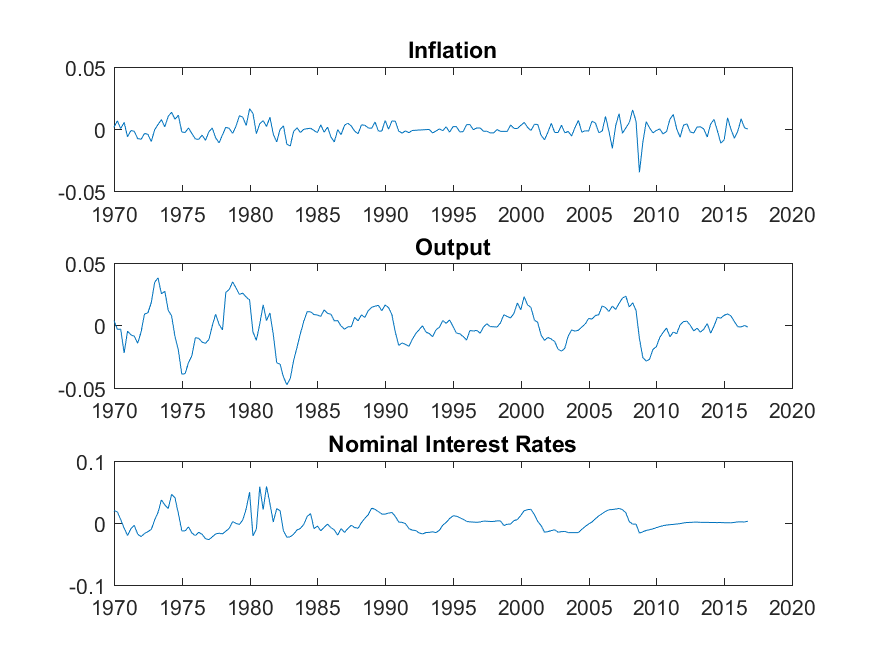
\includegraphics[width=\linewidth]{data}
	\caption{FRED Detrended Data}
	\label{fig:data}
\end{figure}

Note that the values for $\sigma$ for our simulation somewhat matches the data. This might imply reasonable parameters values for our model.

\begin{table}[H]
	\centering
\begin{tabular}{c|c|c}
	\hline 
	& Simulation & Data \\ 
	\hline 
	$\sigma_{\pi}$ & 0.0070    &  0.0060  \\ 
	$\sigma_{y}$ & 0.0113    & 0.0150 \\ 
	$\sigma_{i}$ &   0.0147 &  0.0154\\ 
	\hline 
\end{tabular} 
	\caption{Standard deviation of inflation, output and interest rate}
\label{tab:sigma}
\end{table}
\section*{Part (e)}

Note that we can write our model in the following state space form

Then, we can write inflation, output and nominal interest rates in the following matrix form
\begin{align*}
S_t &= A S_{t-1} + C \epsilon_t\\
Z(t) &= DX(t)
\end{align*}
where $A$ and $C$ are defined as previously, $\epsilon_t\sim N(0,I)$, and
\[
D = \bmat{0& 1& 0& 0& 0& 0& 0& 0& 0\\
	1& 0& 0& 0& 0& \psi_{ya}& 0& 0& 0\\
	0 &0& 0& 1& 0& 0& 0& 0& 0}
\]

Using the Kalman filter code from the last problem set we can compute $S_t$. In Fig.\ref{fig:kalman}, we report both the ouput and the output gap.
\begin{figure}[H]
	\centering
	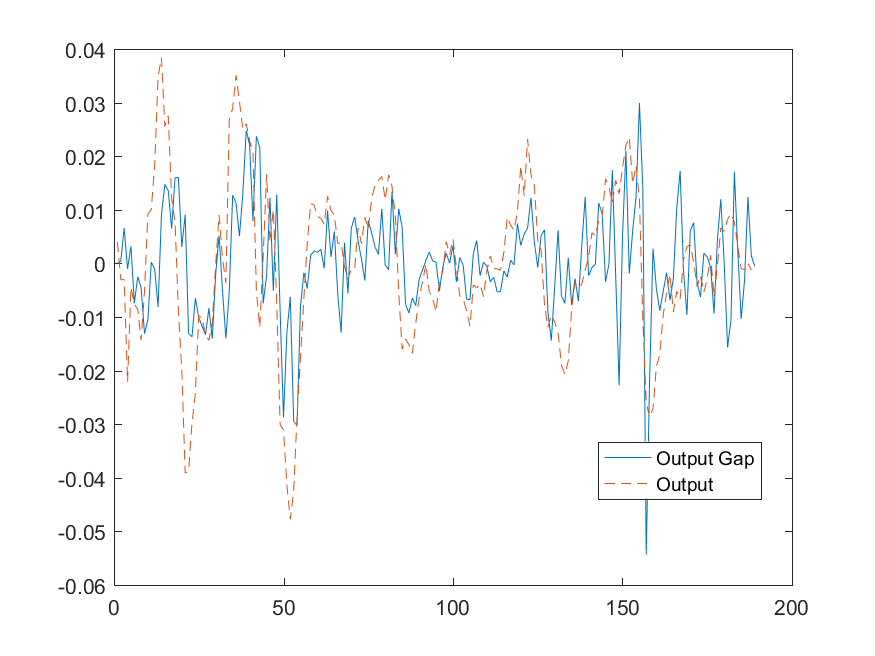
\includegraphics[width=\linewidth]{kalman}
	\caption{Kalman Filter estimate of output and output gap}
	\label{fig:kalman}
\end{figure}

As seen in Fig.\ref{fig:kalman}, the output gap follows output closely. This implies that $y_t^n-y$ is fairly close to 0 for all $t$. Is it reasonable? It seems unlikely that the natural level of output should always be close to the trend as we expect shocks in productivity to push $y_t^n$.

\section*{Code}
\lstinputlisting[language=Matlab]{main.m}
\subsubsection*{Kalman Filter (kfilter.m)}
\lstinputlisting[language=Matlab]{kfilter.m}

\end{document}
